% !Mode:: "TeX:UTF-8"

\BiChapter{密集热点区域无线网络的研究基础}{architecture and system model}

本章介绍密集热点区域无线网络研究的基础知识,首先介绍了超密集组网的定义,
接着介绍超密集组网场景中可能用到的网络架构,
其中包括CRAN架构和多用户多点联合传输架构,
最后介绍无线网络分析的的重要的性能指标。
为接下来的理论分析和算法优化打下基础。

\BiSection{超密集组网的定义}{Defination of UDNs}

超密集组网技术是5G中的关键的技术,用于满足大量用户的区域内,用户的高速率传输的需求\citeup{edgeudn}。
密集热点区域无线网络场景下,由于系统中的用户较多,容量需求大,因此,需要网络能够提供更高的单位面积的频谱利用率\citup{datamaxudn}。
同时,通信已经成为世界上最耗能的应用\citeup{costudn},因此要想办法在满足用户要求的同时,尽可能的降低能耗,从而得到较高的能耗比,即网络需要有很高的单位面积能量谱效率。

超密集组网(UDN)作为~5G~的关键技术之一,对其概念的描述,网络布置的探索,再到性能分析、具体干扰管理算法的研究,随着对~5G~标准的不断探索,这些方面的研究也越来越深入。
未来通信系统服务需求的增加,且需要满足更好的用户体验,系统容量的增加就显得日益迫切。

根据现有的研究结果进行分析,超密集组网~UDN~在~5G~中的定义是:发射功率较低的小型的接入点,网络的拓扑结构不做精确的规划要求,网络中基站的密集程度很高的区域部署,即可以构成一个超密集网络\citeup{5Gwhitebook}。
采用超密集组网技术,发射机和接收机之间的距离大大降低,减少了路径损耗,单位面积内可以服务的用户量大大增多,提高频谱效率,小区中的流量的分配更加灵活,有效的提升了网络效率\citeup{spsharing} 。
总结来说,超密集组网就是通过提高单位面积频谱效率的方式来提高整体的系统容量\citeup{channeludn}。
超密集网络中单个小区提升系统容量的方式又分为以下两种:其一为增加带宽,为现有网络提供新的频谱资源;
其二为使用 Massive MIMO、高阶调制等方式提高每个小区的频谱效率。
超密集组网的网络部署方式仍处于探索阶段,但有几点已经达成共识。
第一,单一层次的蜂窝网部署方式无法满足 5G 移动通信系统的通信需求,多层次、多种接入方式并存的无线接入网络(Heterogeneous and Small Cell Networks, HetSNets)
是蜂窝网发展的必然趋势。
多层次是指传统宏小区(Macrocell)和包括微小区(Picocell)、家庭小区(Femtocell)、中继(Relay Nodes)在内的低功耗小区共存的体系结构。
除了传统蜂窝网接入方式以外,也包括无线局域网、无线个域网等多种接入技术。
第二,办公区域、居住区域、旅店商场等室内热点区域以及机场等室外热点区域需要高密度的小区部署,从而支持满足 QoS 要求的用户服务。
第三,除了手机等蜂窝网用户设备(UE)以外,还需要支持机器间通信,这种通信
业务也要与核心网络相连。
同时,对于大量的微小基站的接入,光纤和无线都应该被认为是合适的传输资源。

UDN 需要以非常灵活的方式来使用各类传输资源,如有线传输,无线传输,或混合传输,这样才能从时域,频域,空域等各个维度来全面地利用传输,以达到对资源的最大使用效率。
UDN 的网络拓扑结构应该是灵活的,以便动态地适应各种热点地区的部署,适应大量网络节点的接入,并适应多种无线技术。
因此,先进的自配置算法将被大量地使用在 UDN 网络中,以获得自动的小区参数配置,自动容量优化,自动负载平衡,自动资源分区及自主协调等能力。

\BiSection{超密集组网的网络架构}{The construction of UDN}
本小节中介绍超密集组网网络架构中较有潜力的,可以被应用的具有前景的网络架构,其中包括异构网络架构、CRAN架构和SDN架构。

\BiSubsection{CRAN}{CRAN}
C-RAN架构最大的特点是基带资源池化特性,基带资源可以在不同的基站之间共享。
基于虚拟基带处理单元池和遥控射频端的联合,相比于其他的蜂窝网络,C-RAN架构有更低的网络延时。
CRAN~网络架构如图~\ref{CRAN}~所示。
\begin{figure}[htbp]
\centering
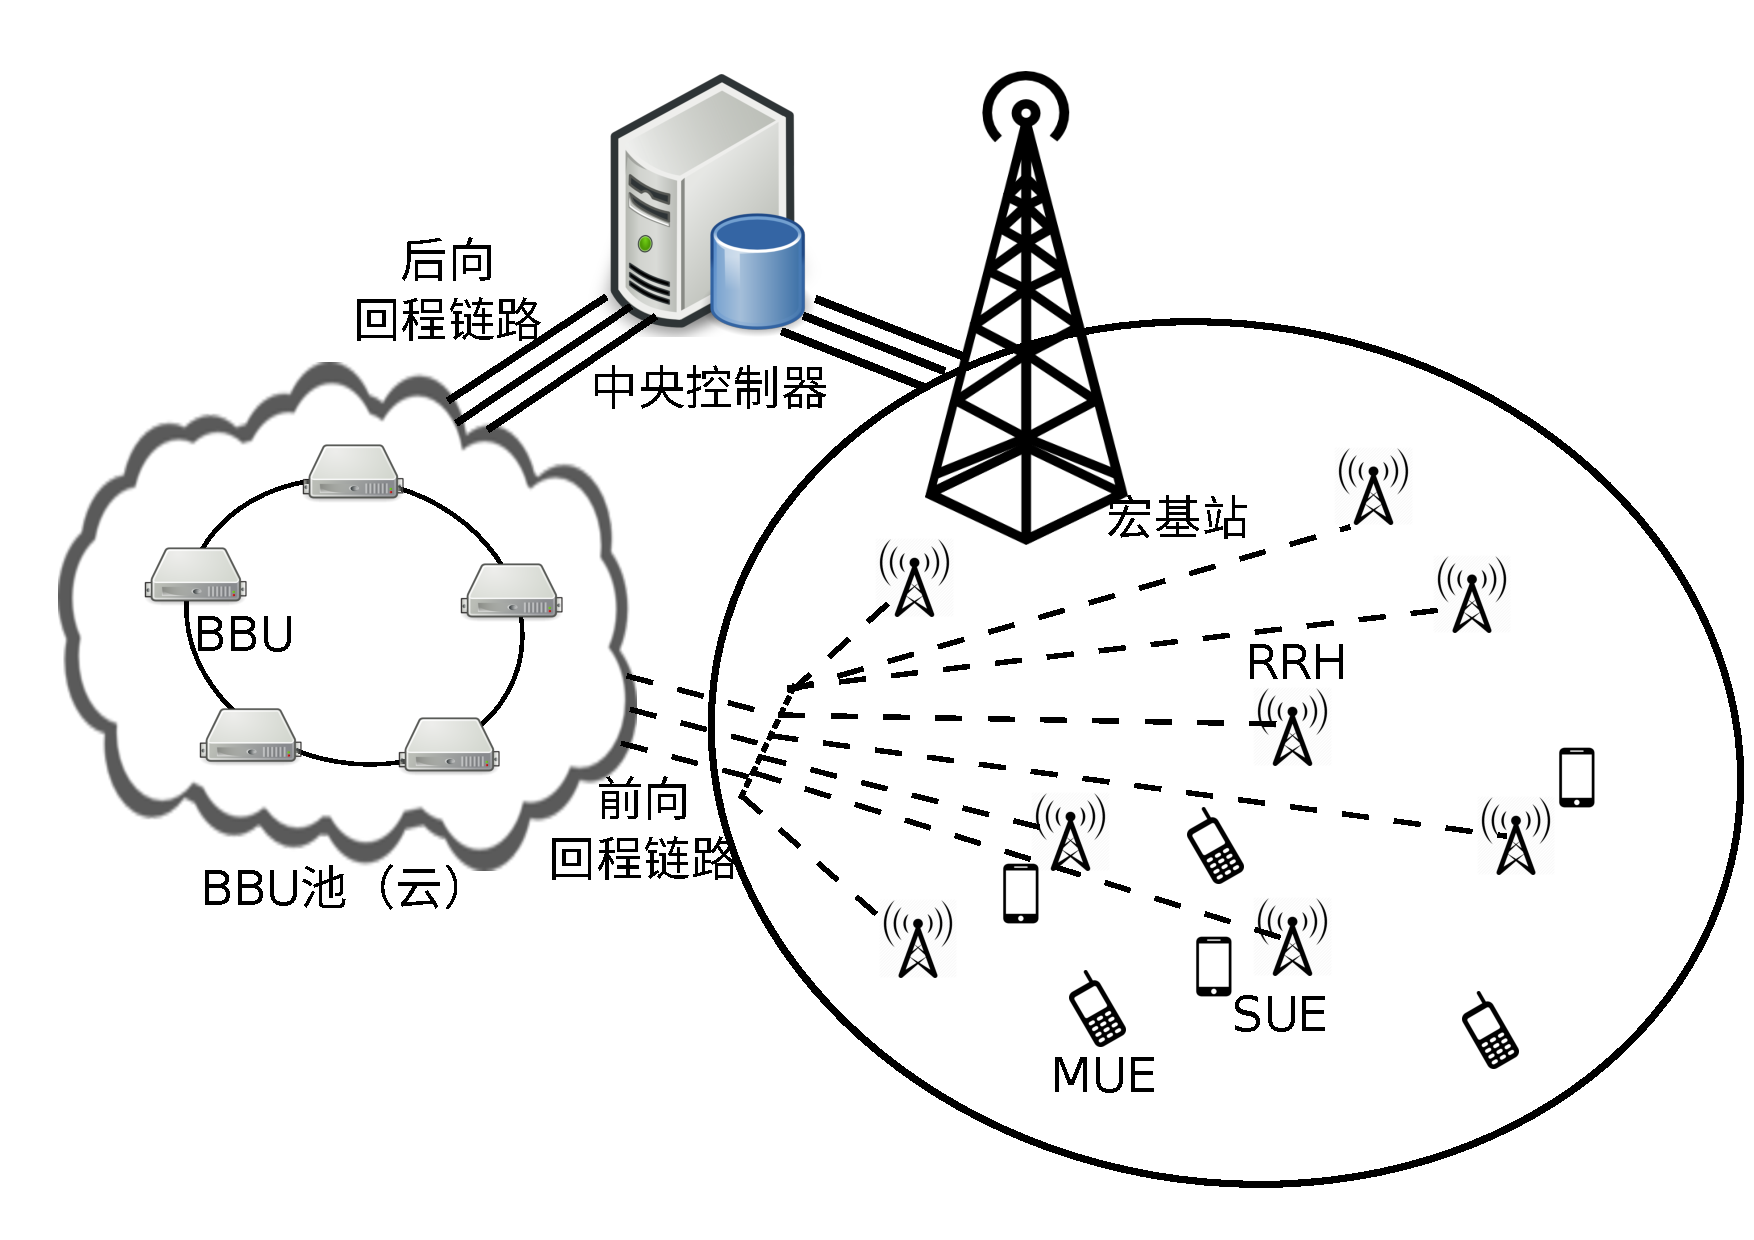
\includegraphics[width = 0.62\textwidth]{H-C-RAN_PPP.pdf}
\caption{CRAN~网络架构的示意图}\vspace{-1.5em}
\label{CRAN}
\end{figure}
从图~\ref{CRAN}~中可以看出,网络主要有三个部分组成,分别为中央控制器,基带处理单元池(~BBU~)池
遥控射频头(~RRH~),~BBU~池通过后向回程链路(~Backhaul~)与中央控制器相连接,
通过前向回程链路(~Fronthaul~)与~RRH~相连接。
再一次下行通信中,中央控制器主要完成网络层上的协议,如小区切换、跨区访问等\citeup{greencran}。
信号经过网络层的处理通过后向回程链路下发到物理层,
由~BBU~池完成基带信号的处理,其中包括小区分簇\citeup{clustercran}、多用户联合传输\citeup{compcran}、预编码\citeup{mmimocran}、调制、信道编码等\citeup{jthcran}。
经过基带处理的信号通过前向回程链路传输到~RRH,在~RRH~上完成数模转换和功率放大等射频端的过程。
上行链路的通信是下行链路的逆过程,每个部分完成的功能也大致相同。
CRAN~通过将网络层、基带处理、射频处理三者分离,将需要运算复杂度较高的基带处理部分从基站端剥离,
将多个基站的基带信号处理单元放置在云端,将最新的云计算技术应用到信号处理当中,
网络的运算能力大大增强\citeup{d2dcran2}。
除此之外,由于云端的~BBU~池与小区内的微基站~RRH~均进行了连接,
因此可以将小区内的微基站的新到状态信息汇总,使得最新的分布式的技术,如分布式~MIMO技术、
分布式预编码技术的使用成为了可能。

CRAN是干扰协调和频谱资源管理的有效的方法。由于RRH结构简单,RRH可以以较低的硬件成本进行密集的布放,BBU池化后资源统一调度,能量效率更高。
由于中心化的架构,多用户干扰可以被诸如CoMP这样的多点协作技术有效的解决掉,这样将会有很有效的性能增益。
在传统的CRAN架构中(4G),C-RAN被部署用于连接宏基站和BBU池,由于BBU和RRH之间的传输路径长,这种传统的基站会造成很大的传输时延,而在密集热点区域采用C-RAN架构,延迟也会被大大的缩短。
不仅如此,它还是有效解决潮汐效应的一种方式\citeup{interference_lim_cran}。

但CRAN架构也不是完美的。若要将CRAN架构应用于超密集组网当中,需要减小功耗\citeup{icccran},建立RRH睡眠与活跃状态的选择机制。
不仅如此,还要实现低花费的前向链路,因为前向链路能够提供的能量资源是有限的。
同时也要降低网络中算法的复杂度,降低训练开销。

\BiSubsection{多用户联合传输技术}{CoMP}

联合传输技术(~CoMP~)最早有3GPP提出\citeup{jointaseeeopt},应用联合传输技术,
基站通过后向回程链路相互连接在一起\citeup{compund2},
同时为用户提供服务,在多用户联合传输系统下,基站可以采用预编码等技术为多个用户同时提供服务。

联合传输技术是伴随第四代移动通信~(4G)~提出的一个关键技术\citeup{compca}。
其主要的思想是以用户为中心,将基站联合起来,进行协作,
共同对用户进行服务\citeup{uplinkcomp}。
由于基站间相互联合共同服务区域内的用户用户,
处在基站边缘的用户的干扰功率也能被用户利用成为有用的接收功率,从而使得边缘用户的有效性大大提升\citeup{compudn3}。
联合传输的架构示意图如图~\ref{CoMP}~所示,
\begin{figure}[htbp]
\centering
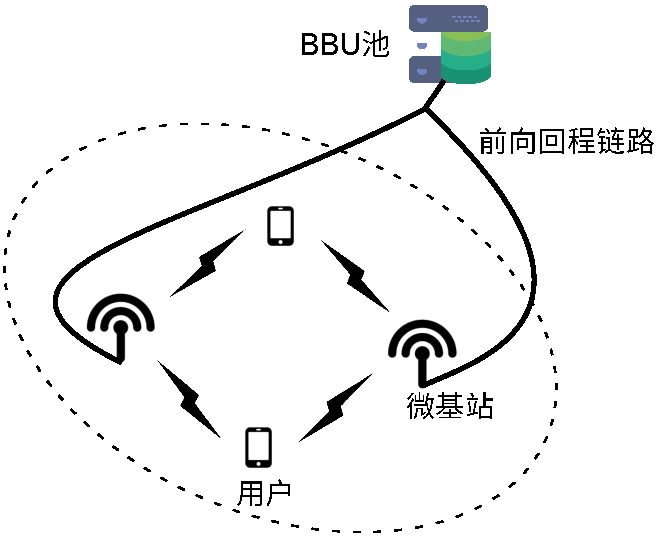
\includegraphics[width = 0.62\textwidth]{CoMP.pdf}
\caption{联合传输网络架构示意图}\vspace{-0.5em}
\label{CoMP}
\end{figure}
从图中可以看到,网络由用于处理数字信号的BBU池,用户传输信号的微基站和前向回程链路组成。
传送给用户的信息首先通过BBU池进行数据处理,在通过前向回程链路传输到基站端,由于采用了干扰消除算法,因此两个基站传送给用户的信息均为用户可以利用的有效信号,
实现两个基站联合传输共同服务区域内的用户的目的。


\BiSection{超密集组网通信的性能指标}{matrices}
本小节介绍衡量超密集组网的通信性能的主要指标,其中包括信干噪比、遍历容量、覆盖率和单位面积谱效率。

\BiSubsection{信干噪比}{SINR}

可靠性和有效性一直是评定通信性能的一个重要指标。其中有效性可以通过网络的信道容量进行衡量。而网络的信道容量是一个直接与信干噪比有关的量。
信干噪比的表达式如~(\ref{SINR})~所示:
\begin{equation}\label{SINR}
  \mathrm{SINR}=\frac{S}{I+N}
\end{equation}
其中~$S$~为通信链路中接收机的接收功率,~$I$~为其他的通信链路对该通信链路所造成的干扰。$\mathrm{SINR}$~表示该通信链路的信干燥比。

超密集组网区域用户与基站之间距离比较近,因此干扰占有几乎全部的比重,反之噪声的影响几乎可以忽略不计。也就是说,密集无线网络是一个干扰受限的信道。其信干比近似等于信干燥比。信干比的表达式如~(\ref{SIR})~:
\begin{equation}\label{SIR}
  \mathrm{SIR}=S/I
\end{equation}
其中~$\mathrm{SIR}$~表示该通信链路的信干比。
\BiSubsection{用户的遍历容量}{ASE}
给定一个用户的接收信干比,即可以求出一个用户的遍历容量,在平稳的瑞利信道下,用户的遍历容量如式~$\ref{e_capacity_formular}$~所示:
\begin{equation}\label{e_capacity_formular}
  C_{Rayleigh} = \int_{0}^{\infty} B \log_2(1+\mathrm{SINR}(h)) f(h) \mathrm{d} h
\end{equation}
其中~$C_{Rayleigh}$~为瑞利信道的遍历容量,~$f(h)$~为~$h$~的概率密度分布函数,$B$~为信道的带宽。信道的遍历容量表示一个用户在一段时间内,遍历所有可能性下的信道容量的统计平均值。
因为信道为瑞利信道,因此在固定位置上的用户,由于受到了信道系数的影响,其信干噪比在不同的时间点上也是不同的,又由于瑞利信道是平稳的信道,
因此可以采用遍历所有信道系数的可能性得到的统计均值代替时间上的遍历,用~$\mathrm{SINR}(h))$~表示。

遍历容量可以反应一个用户在一段时间内通信的有效性,是反应网络性能的重要指标。

\BiSubsection{区域覆盖率}{Coverage}
为保证用户的服务质量与速率要求,用户的接收信干比需要维持在一个固定的门限上,而到底有多少用户在该时刻上有很好的信干比,或者说在瞬时上能达到所要求的信干比的用户一共有多少呢?区域覆盖率是评定的有效的指标。
区域覆盖率的定义如~(\ref{pc})~所示:
\begin{equation}\label{pc}
  p_c(T) = \mathbb{P}[\mathrm{SINR}>T]
\end{equation}
其中~$T$~为给定的信干噪比的门限,~$\mathrm{SINR}$~为通信链路的信干噪比,$\mathbb{P}$~表示概率。根据定义,可对其物理意义做出以下的三种解释:

 (1)~服务用户的信干噪比为以上的概率。

 (2)~信干噪比为以上的用户占总用户的百分比。

 (3)~信干噪比为以上的区域占总区域的百分比。

覆盖率是评定无线网络性能的一个重要的概念,并且根据覆盖率,可以很容易的得到有能达到给定的速率要求在整个区域中的所有用户的占比。
同时该物理量也是单位区域上信干噪比的概率分布函数的补函数。
\BiSubsection{区域面积谱效率}{ASE}

香农定理给出了通信系统的理论容量上界\citeup{TheMathematicalTheoryOfCommunication},表达式如~(\ref{shannon})~所示:
\begin{equation}\label{shannon}
  C = B \log_2(1+\mathrm{SINR})
\end{equation}

式~(\ref{shannon})~中,~$C$~ 代表理论的容量的上界也即系统最大的传输速率, $B$ 代表信道的带宽, ~$\mathrm{SINR}$~ 代表接收端信号的信干噪比。
香农定理可以解释现代各种无线制式由于带宽不同,所支持的单载波最大吞吐量的不同。香农公式表达了在给定带宽下,噪声和干扰都服从高斯分布的情况下,系统所能达到的理论最大容量。

频谱效率的定义为单位带宽上所能承载的最大的吞吐量,如~(\ref{SE})~所示:
\begin{equation}\label{SE}
\eta_{SE}=C/B=\log_2(1+\mathrm{SINR})
\end{equation}
上式中~$C/B$~就是单位带宽的容量,单位为~$bps/\mathrm{Hz}$~体现信道链路的传输性能。式~(\ref{SE})~给出了理论上频谱效率的理论最大值。

在密集热点区域无线网络的场景中,单个链路的容量已经不再是衡量一个网络的好坏的唯一指标,在超密集热点区域无线网络的场景中,还要考虑在一段时间内,网络中服务的用户的和容量。
同时,考虑到不同区域上的频谱效率相差可能非常悬殊。因此在密集热点的网络环境下,频谱效率将不能够完全反映整个区域的无线网络的性能,
取而代之的是单位面积谱效率这一物理量,其定义为在单位面积上的频谱效率,表达式如~(\ref{ASE})~所示:
\begin{equation}\label{ASE}
  \eta_{ASE}=C/(B\cdot S) = \lambda\mathbb{E}[\log_2(1+\mathrm{SINR})]
\end{equation}
单位为~$bps/\mathrm{Hz}/\mathrm{m}^2$~。其中~$\lambda$~为服务区域内基站的密度。区域面积谱效率的物理意义为单位面积上所承载的平均的和容量。

\BiSection{本章小结}{Conclusion}
本章主要对超密集组网现阶段的研究基础进行了分析,为后续章节的深入分析打下基础。
首先给出了超密集组网的定义,在分层异构的网络架构下,通过部署高密度低功耗的节点,来极大的提升系统容量,达到下一代移动通信 5G 满足1000 倍速率提升的要求。
同时给出通信性能的衡量指标,一般通过区域频谱效率,区域能量效率,成本效率来衡量超密集组网。
核心性能指标和典型场景指标则从实用性的角度给出了系统需要符合的性能参数,对于实际系统的规划与部署具有指导意义。
为了进一步明确超密集组网的网络构架,多址接入技术以及实现大容量的可行性,本章的第三部分给出了超密集组网中的主要技术,大规模天线技术可以带赋形增益和频谱效率的提升;
新型的非正交稀疏码分多址技术 SCMA 可以在利用同等资源的情况下,接入更大量的用户,提升系统容量;
以去蜂窝网化为核心理念的 C-RAN 技术,可以进行信息的集中处理,降低能耗;
D2D 技术作为超密集组网中最具潜力的技术,使得大规模密集通信成为可能。
文章对这四种技术进行简要介绍和说明,确定在超密集组网中的使用方式,所能取得的性能优势。
